\documentclass[12pt]{article}
\usepackage[top=1in,left=1in, right = 1in, footskip=1in]{geometry}

\usepackage{graphicx}
%\usepackage{adjustbox}

%% \newcommand{\comment}{\showcomment}
\newcommand{\comment}{\nocomment}

\newcommand{\showcomment}[3]{\textcolor{#1}{\textbf{[#2: }\textsl{#3}\textbf{]}}}
\newcommand{\nocomment}[3]{}

\newcommand{\jd}[1]{\comment{cyan}{JD}{#1}}
\newcommand{\swp}[1]{\comment{magenta}{SWP}{#1}}

\newcommand{\eref}[1]{(Eq.~\ref{eq:#1})}
\newcommand{\fref}[1]{Fig.~\ref{fig:#1}}
\newcommand{\Fref}[1]{Fig.~\ref{fig:#1}}
\newcommand{\sref}[1]{Sec.~\ref{#1}}
\newcommand{\frange}[2]{Fig.~\ref{fig:#1}--\ref{fig:#2}}
\newcommand{\tref}[1]{Table~\ref{tab:#1}}
\newcommand{\tlab}[1]{\label{tab:#1}}
\newcommand{\seminar}{SE\mbox{$^m$}I\mbox{$^n$}R}

\usepackage{amsthm}
\usepackage{amsmath}
\usepackage{amssymb}
\usepackage{amsfonts}

% \usepackage{lineno}
% \linenumbers

\usepackage[pdfencoding=auto, psdextra]{hyperref}

\usepackage[numbers]{natbib}
\usepackage{hyperref,url}
\bibliographystyle{unsrt}
\date{\today}

\usepackage{xspace}
\newcommand*{\ie}{i.e.\@\xspace}

\usepackage{color}

\newcommand{\Rx}[1]{\ensuremath{{\mathcal R}_{#1}}} 
\newcommand{\Ro}{\Rx{0}}
\newcommand{\RR}{\ensuremath{{\mathcal R}}}
\newcommand{\Rhat}{\ensuremath{{\hat\RR}}}
\newcommand{\tsub}[2]{#1_{{\textrm{\tiny #2}}}}

\begin{document}

\begin{flushleft}{
	\Large
	\textbf\newline{
		Potential roles of social distancing in mitigating the spread of coronavirus disease 2019 (COVID-19) in South Korea
	}
}
\newline
\\
Sang Woo Park\textsuperscript{1,*}
Kaiyuan Sun\textsuperscript{2}
C\'ecile Viboud\textsuperscript{2}
Bryan T.\ Grenfell\textsuperscript{1,2,3}
Jonathan Dushoff\textsuperscript{4,5,6}
\\
\bigskip
\textbf{1} Department of Ecology and Evolutionary Biology, Princeton University, Princeton, NJ, USA
\\
\textbf{2} Fogarty International Center, National Institutes of Health, Bethesda, MD, USA
\\
\textbf{3} Woodrow Wilson School of Public and International Affairs, Princeton University, Princeton, NJ, USA
\\
\textbf{4} Department of Mathematics and Statistics, McMaster University, Hamilton, ON, Canada
\\
\textbf{5} M.\,G.\,DeGroote Institute for Infectious Disease Research, McMaster University, Hamilton, ON, Canada
\\
\textbf{6} Department of Biology, McMaster University, Hamilton, ON, Canada
\\
\bigskip

*Corresponding author: swp2@princeton.edu\\
This article does not necessarily represent the views of the NIH or the US government.
\end{flushleft}

\section*{Abstract - 75 word limit; currently 70.}

On January 20, 2020, the first COVID-19 case was confirmed in South Korea.
As of March 18, 2020, 8,413 cases were confirmed but the number of cases has been consistently decreasing;
the reason for the decrease has been widely attributed to its intensive testing.
We report on the potential roles of social distancing in reducing transmission in South Korea.
Our analysis suggests that transmission may still persist in some regions.

\pagebreak

Since its first appearance in Wuhan, China, in December 2019 \citep{pneumonia}, the novel coronavirus disease (COVID-19) has spread internationally, including to South Korea.
The first COVID-19 case in South Korea was confirmed on January 20, 2020, from a traveling resident of Wuhan, China \citep{kcdc}.
In February, the disease spread rapidly within a church in the city of Daegu.
The chains of transmission that began from this cluster distinguish the epidemic in South Korea from that in any other countries:
As of March 18, 2020, 8,413 cases were confirmed, of which 60\% were related to the church and 27\% were in their 20's \citep{kcdc}.
Nonetheless, South Korea's intensive testing using novel contact tracing techniques allowed rapid identification and isolation cases and reduction of onward transmission \citep{fergusonimpact, tracingkorea, science}.
Here, we describe potential roles of social distancing in mitigating the spread of COVID-19 by using metro traffic data to compare epidemics in two geographically separated major cities in South Korea.

\section{Data description}

We analyzed epidemiological data describing the COVID-19 outbreak in South Korea between January 20--March 16, 2020.
Daily number of reported cases in each geographic region was transcribed from press releases by Korea Centers for Disease Control and Prevention (KCDC) \cite{kcdc}.
Partial line lists were transcribed from press releases from KCDC and various local and provincial governments.
All data and original reports are stored in a publicly available GitHub repository: \url{https://github.com/parksw3/COVID19-Korea}.

\begin{figure}[!h]
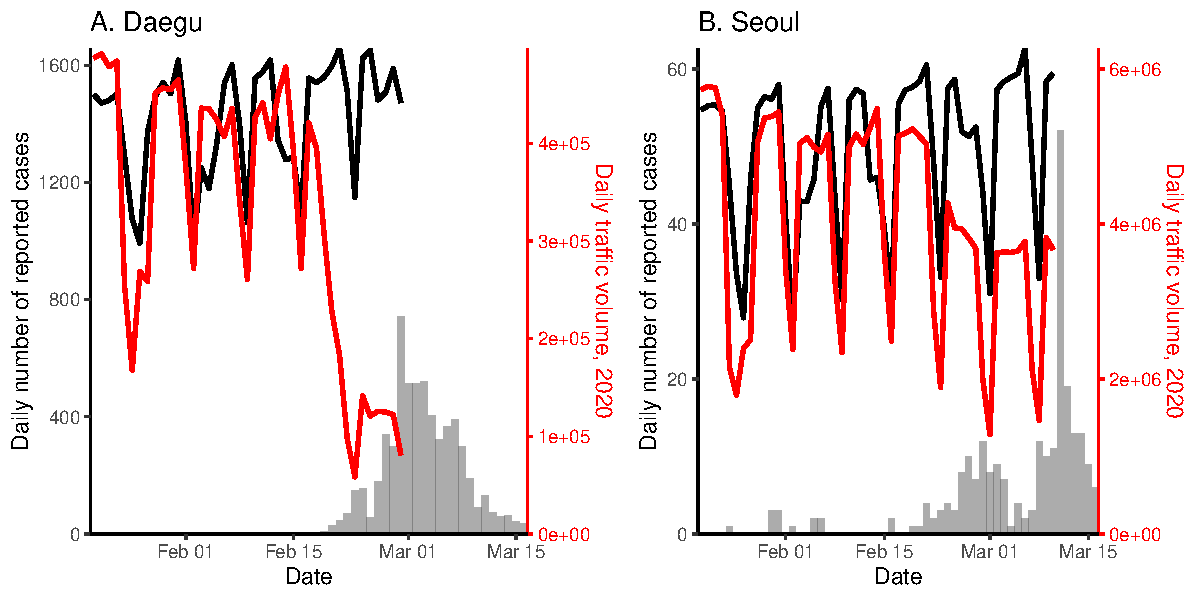
\includegraphics[width=\textwidth]{figure_compare_report.pdf}
\caption{
\textbf{Comparison of epidemiological and traffic data from Daegu and Seoul.}
Solid lines represent the daily metro traffic volume in 2020 (red) and mean daily traffic volume between 2017--2019 (black).
Daily traffic from previous years have been shifted by 1--3 days to align day of the weeks.
Vertical lines indicate Feb 18, 2020, when the first case was confirmed in Daegu.
}
\label{fig:data}
\end{figure}

We compared epidemiological dynamics of COVID-19 from two cities in which the biggest number of COVID-19 cases have been reported: Daegu and Seoul.
Between January 20--March 16, 2020, 6,083 cases from Daegu and 248 from Seoul were reported by the KCDC (Supplementary Materials).
Unlike the epidemic in Daegu, which is characterized by a single, large peak followed by a gradual decrease, the epidemic in Seoul consists of several small outbreaks (\fref{data}).

Daily metro traffic in Daegu and Seoul between 2017--2020 was obtained from \url{data.go.kr} and \url{data.seoul.go.kr}, respectively.
We tabulated the total number of individuals who accessed subway or monorail (\fref{data});
we restricted our analysis to subway lines 1--9 in Seoul.
Soon after the first church-related case was confirmed in Daegu on Feb 18, 2020, the daily traffic volume decreased by about 80\% and 50\% in Daegu and Seoul, respectively.

%% https://www.data.go.kr/dataset/15002503/fileData.do
%% https://data.seoul.go.kr/dataList/OA-12914/S/1/datasetView.do

\section{Trends in time-dependent reproduction number and traffic volume}

\begin{figure}[!ht]
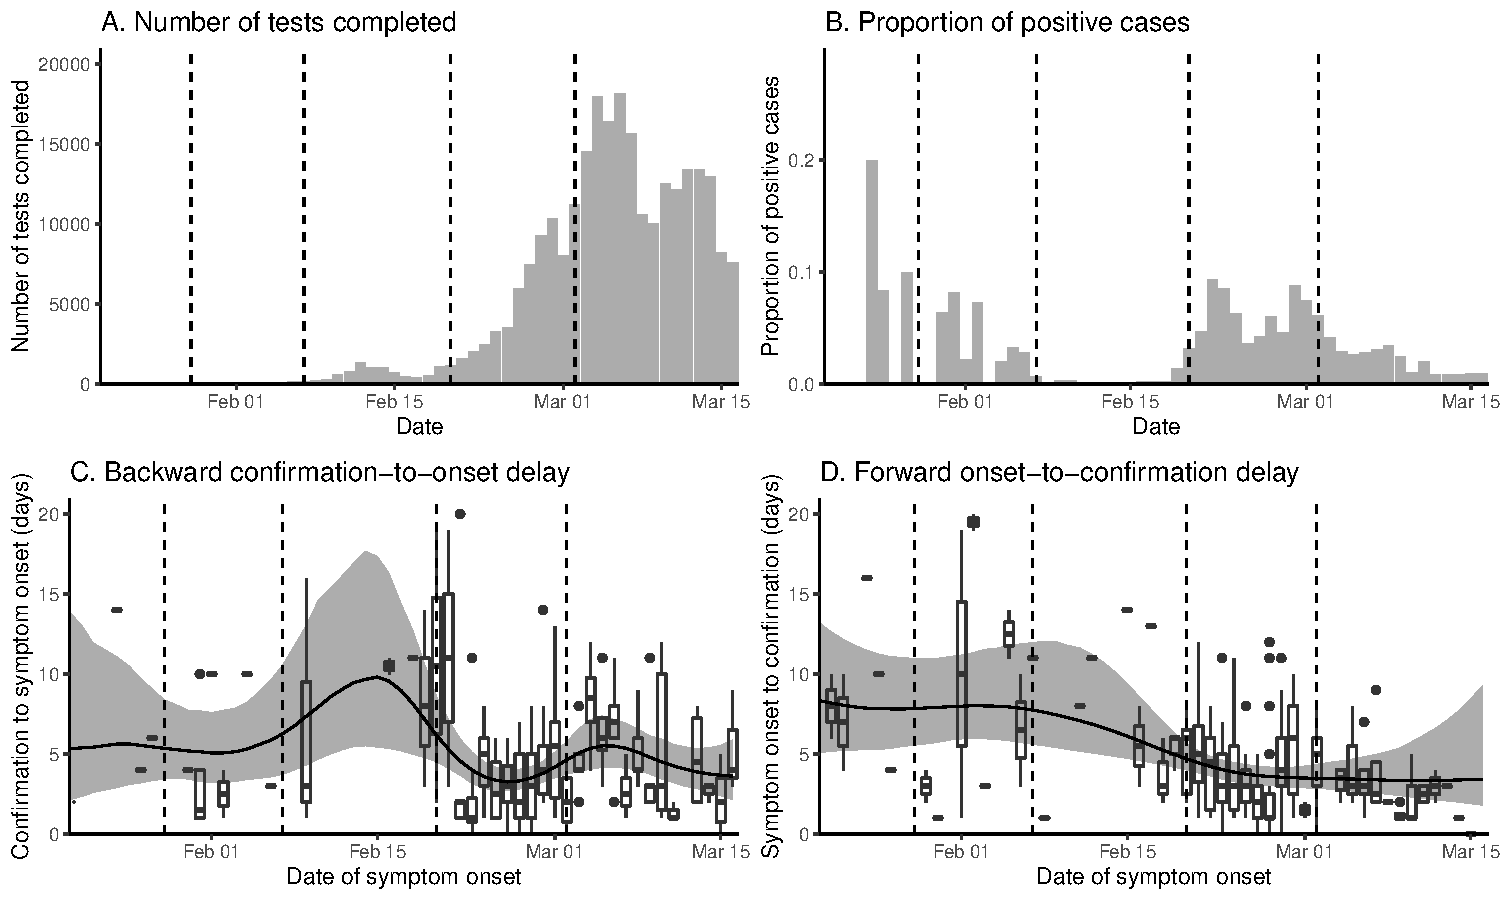
\includegraphics[width=\textwidth]{figure_report_delay.pdf}
\caption{
\textbf{Changes in the number of tests and delay distributions over time.}
}
Vertical lines indicate the date on which testing criteria expanded.
Boxplots (C--D) represent the observed delays.
Black lines and gray ribbons represent the median estimates of the mean delays and their associated 95\% credible intervals.
\label{fig:dist}
\end{figure}

In order to estimate the time-dependent reproduction number $R_t$ (i.e., the expected number of secondary cases caused by an individual infected at time $t$ \citep{fraser2007estimating}), we reconstructed the incidence time series (i.e., the number of infected individuals on each day) from the daily number of reported cases by the KCDC \citep{kcdc}.
We first adjusted the number of reported cases to account for changes in testing criteria (\fref{dist}), which occurred 4 times between January 20--March 16, 2020, as well as changes in the number of tests (Supplementary Materials).
A sensitivity analysis showed that qualitative patterns of inferred $R_t$ are robust to these adjustments.

We then estimated time-dependent \emph{backward} confirmation-to-onset delay distributions from the partial line list using a negative-binomial regression with the \texttt{brms} package \citep{burkner2017brms} (\fref{dist}C).
We combined the estimated posterior distribution of delay distributions with previously estimated incubation period distribution (Table 1) to obtain posterior samples for date of infection for each confirmed case.
Likewise, we estimated time-dependent \emph{forward} onset-to-confirmation delay distribution using the same negative-binomial regression model, while accounting for right-censoring (\fref{dist}D),
to calculate the median probability that a case infected on a given day will be reported before March 16, 2020.
Changes in the mean backward delay (\fref{dist}C) reflect changes in incidence of symptomatic cases, whereas the decrease in the mean forward delay (\fref{dist}D) reflects the improvement in the accuracy of case identification \citep{lai2020effect}.
Implementation details are provided in the Supplementary Materials.

\begin{table}[t]
\begin{center}
\small
\begin{tabular}{p{4cm}|p{4.5cm}|p{4.7cm}|l}
 & Parameterization & Priors & Source \\
\hline
Incubation period\newline distribution & $\mathrm{Gamma}(\mu_I, \mu_I^2/\sigma^2)$ & $\mu_I\sim \mathrm{Gamma}(6.5\,\textrm{days}, 145)$\newline$\sigma\sim \mathrm{Gamma}(2.6, 25)$ & \citep{backer2020incubation} \\
\hline
Generation-interval\newline distribution & $\mathrm{NegativeBinomial}(\mu_G, \theta)$ & $\mu_G\sim\mathrm{Gamma}(5\,\textrm{days},62)$\newline$\theta\sim\mathrm{Gamma}(5,20)$ & \citep{ferretti2020quantifying, ganyani2020estimating} \\
\hline
\end{tabular}
\end{center}
\caption{
\textbf{Assumed incubation and generation-interval distributions.}
Gamma distributions are parameterized using its mean and shape.
Negative binomial distributions are parameterized using its mean and dispersion.
Priors are chosen such that the 95\% quantiles of prior means and standard deviations are consistent with previous estimates.
}
\end{table}

For each posterior sample of the reconstructed incidence time series, we divided daily incidence by the probability that they would have been reported before March 16, 2020, and estimated the time-dependent reproduction number using the renewal equation with a 14-day sliding window \citep{fraser2007estimating}:
\begin{equation}
\mathcal R_t = \frac{I_t}{\sum_{k=1}^{14} I_{t-k} w_k},
\end{equation}
where $I_t$ is the censoring-adjusted incidence time series and $w_k$ is the generation-interval distribution randomly drawn from a prior distribution (Table 1).
We weighted each sample of $\mathcal R_t$ by a gamma probability distribution with a mean of 2.6 and a standard deviation of 2 to reflect prior knowledge \citep{tempvar} and took weighted quantiles to calculate the medians and associated 95\% credible intervals.
We restricted the calculation of $\mathcal R_t$ between February 2, 2020 (14 days after the first confirmed case was imported) and March 10, 2020 (because the degree of censoring would be too large after this date to estimate $\mathcal R_t$).

\begin{figure}[!ht]
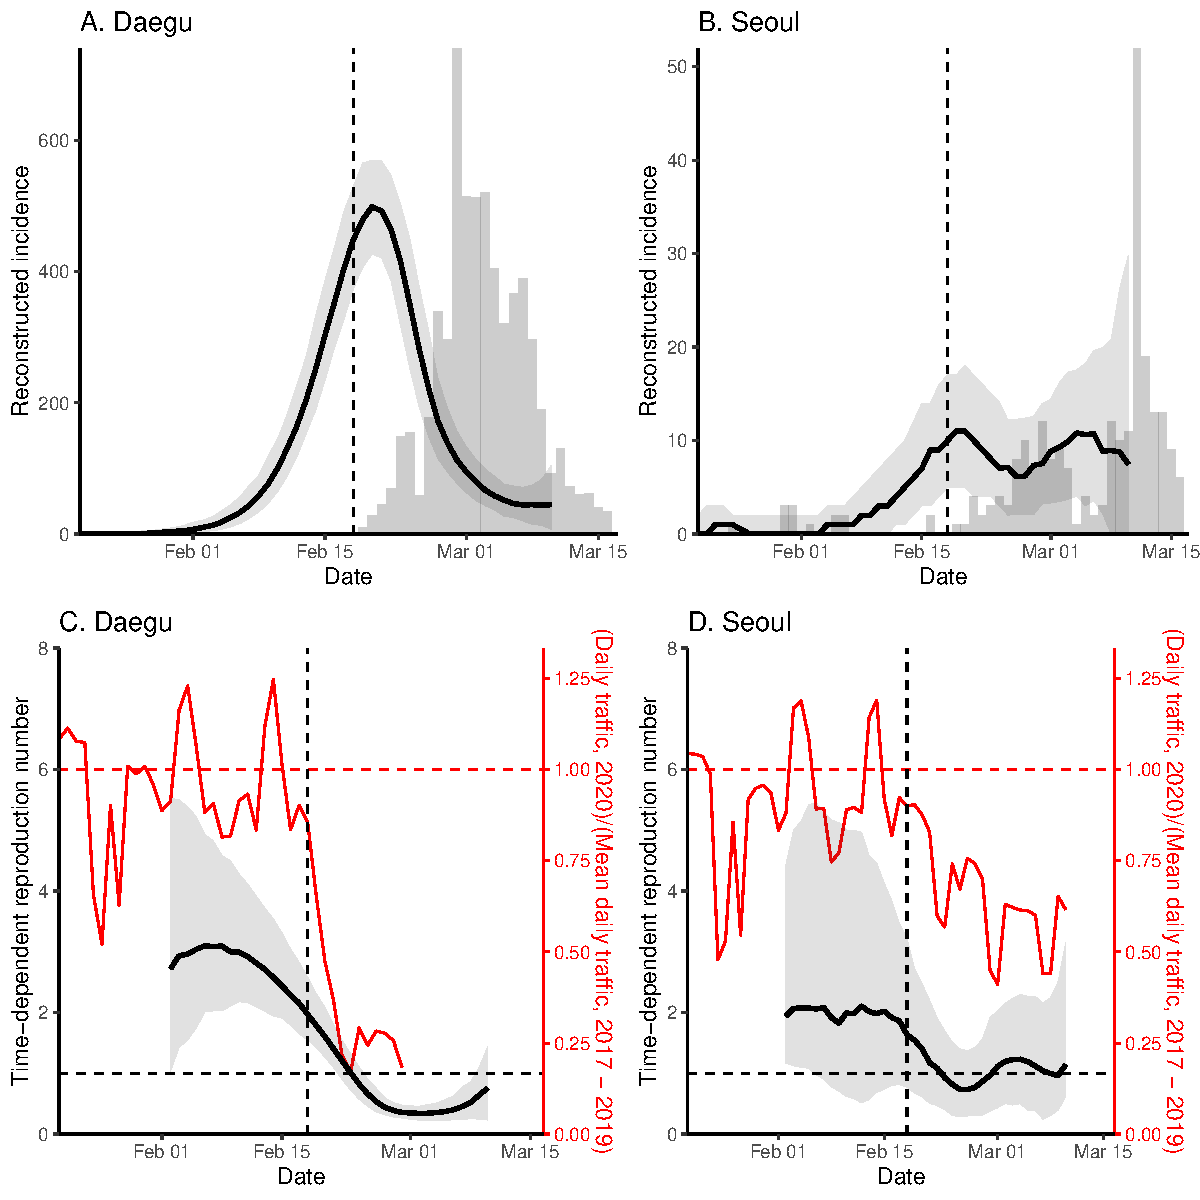
\includegraphics[width=\textwidth]{figure_compare_R_t.pdf}
\caption{
\textbf{Comparison of reconstructed incidence and time-dependent reproduction number in Daegu and Seoul.}
Black lines and gray ribbons represent the median estimates of reconstructed incidence (A,B) and $R_t$ (C,D) and their corresponding 95\% credible intervals.
Red lines represent the normalized traffic volume.
Vertical lines indicate Feb 18, 2020, when the first case was confirmed in Daegu.
}
\label{fig:eff}
\end{figure}

\fref{eff} compares the reconstructed incidence (A,B) and estimates of $\mathcal R_t$ (C,D) in Daegu and Seoul.
In Daegu, estimates of $\mathcal R_t$ gradually decrease and eventually drop below 1 about a week after the reporting of its first case, coinciding with the decrease in the metro traffic volume (\fref{eff}C).
The initial decrease in $\mathcal R_t$ may reflect the possibility that a large proportion of church-related transmission could have occurred much earlier and therefore caused behavior change within the church; for example, the first confirmed case in Daegu became symptomatic on February 7, 2020, and visited the church on February 9 and 16, 2020 \citep{kcdc}.
% Our estimates of $\mathcal R_t$ for Daegu are consistent with the estimates of $\mathcal R_t$ for South Korea by Abbott \textit{et al.} \cite{tempvar} --- their estimates drop below 1 slightly later because they rely on number of symptomatic cases instead.

On the other hand, estimates of $\mathcal R_t$ remain around 1 in Seoul (\fref{eff}D).
Our analysis suggests that social distancing in Seoul was less intense, and this could be why reduction in spread was less effective.
Stronger distancing or further intervention will be necessary to reduce $\mathcal R_t$ below 1.

While we find clear, positive correlations between the normalized traffic and the median estimates of $\mathcal R_t$ in both Daegu ($r=0.87$; 95\% CI: 0.74--0.94) and Seoul ($r=0.55$; 95\% CI: 0.27--0.74), the strength of correlations are likely to be strongly conflated because they do not account for the effects of any other measures that could have affected $\mathcal R_t$;
in particular, the increase in the number of tests (\fref{dist}A) as well as the improvement in the accuracy of case identification (\fref{dist}D) are likely to have played important roles in reducing $\mathcal R_t$.
We do not find any signatures of lags (Supplementary Materials).
Similar patterns in the estimates of $\mathcal R_t$ are found in directly surrounding provinces (Gyeongsangbuk-do and Gyeonggi-do), providing support for the robustness of our analysis (Supplementary Materials).

\section{Discussion}

The ongoing COVID-19 outbreak in South Korea provides a unique perspective to understanding and controlling the pandemic.
Its experience provides evidence that the epidemic can be suppressed with less extreme measures than those taken by China \citep{kickbusch2020response}.
Our analysis reveals potential roles of social distancing in mitigating the COVID-19 epidemic in South Korea.
Even though social distancing alone may not be able to fully prevent the spread of the disease, its ability to flatten the epidemic curve (cf. \fref{eff}B) reduces burden for healthcare system and provides time to plan for the future \citep{anderson2020will}.

Our study is not without limitations.
In particular, we did not account for differences in the delay distributions or changes in the number of tests among cities.
The intensity of intervention is likely to vary across regions given that majority of COVID-19 cases in South Korea were reported from Daegu.
We did not have the data to account for these factors.
Nonetheless, the robustness of our findings is supported by the sensitivity analyses.
We also did not distinguish local and imported cases, which may overestimate $\mathcal R_t$ \citep{thompson2019improved}. \swp{The analysis of the Seoul outbreak which accounts for imported cases is presented in Supplementary Materials?}

Our analysis focused on comparing metro traffic, which serves as a proxy for the degree of social distancing, with epidemiological dynamics in two cities.
This analysis is indirect; we are not able to directly estimate the effect of social distancing on epidemiological dynamics.
Moreover, other measures, such as intensive testing of core transmission groups and school closure, are also likely to have affected the changes in $\mathcal R_t$ \citep{kcdc}.
Future studies should consider quantifying contributions of different measures in preventing the spread.

Finally, our study highlights the importance of considering geographical heterogeneity in estimating epidemic potential.
The recent decrease in the number of reported cases in South Korea is likely to be strongly correlated with the decrease in the number of cases in Daegu.
Our analysis reveals that the epidemic may still persist in other regions, including Seoul and Gyeonggi-do.
Persistent reportings of COVID-19 cases in Seoul and Gyeonggi-do (around 10 cases almost everyday) between March 11--22, 2020, provide further support for our conclusion \citep{kcdc}.
Unless the reproduction number can be reduced below 1 in all regions, small outbreaks may continue to occur in South Korea.

\section*{Contribution}

Data collection: SWP; conceptualization: SWP, CV; analysis: SWP; first draft: SWP, JD. All authors contributed to the writing and approval of the final report.

\pagebreak

\bibliography{korea}

\pagebreak

\renewcommand\thefigure{S\arabic{figure}}
\setcounter{figure}{0}    

\section*{Supplementary Materials}

\subsection*{Epidemiological data}

The daily number of reported cases from each region was translated and transcribed from the KCDC press release \citep{kcdc}.
Following the KCDC's protocol, the daily number of reported cases prior to February 20, 2020, reflects the number of confirmed cases on each day.
Between February 21 -- March 1, 2020, the daily number of reported cases reflects the number of reported cases within the last 24 hours (9 AM to 9 AM).
On March 2, 2020, the daily number of reported cases reflects the number of cases that were reported between 9 AM March 1, 2020, and 12 AM March 2, 2020.
Since then, the daily number of reported cases reflects the number of reported cases within the last 24 hours (12 AM to 12 AM).
The daily number of reported cases by the KCDC may be different from the reports by each city's government as some cases may be transferred after they are confirmed.

\subsection*{Time series adjustments}

First, we accounted for changes in testing criteria, which occurred 4 times between January 20--March 16, 2020, by assuming that the proportion positive should remain roughly constant if we follow a consistent protocol of identifying and deciding whom to test.
To do so, we calculated the relative proportion of positive cases during each period (divided by the the between-period mean) and multiplied the daily number of reported cases by the relative proportions of the corresponding criterion.
Likewise, we accounted for changes in the number of tests completed on each day by dividing the scaled number of reported cases by the relative number of tests completed on each day; this step was performed separately for each testing criterion because widening of criteria necessarily increases the number of tests.
The number of negative cases was not reported on January 25 and 31, 2020; we took the average of cumulative negative cases from one day before and after these dates instead to impute missing values.

\subsection*{Estimating delay distributions between onset and reporting}

We estimated both forward (onset-to-confirmation) and backward (confirmation-to-onset) delay distributions using Bayesian negative binomial regressions with log links.
The backward delay distribution is inferred directly using the \texttt{brms} package \citep{burkner2017brms}.
The time-dependent mean of the negative binomial distribution is modeled using splines.
We assumed weakly informative priors on the fixed effects: normal distributions with mean of 0 and standard deviation of 2;
note that these distributions are priors on link scale.

To estimate the forward delay distribution, we modified the stan code to account for right-censoring and ran the code using the \texttt{rstan} package \citep{rstan}.
In particular, we modified the likelihood such that given a delay of $x_i$ days, symptom onset day $t_i$ and the day of measurement of $k$, the likelihood of observing the delay is given by:
\begin{equation}
\frac{f(x_i|\mu(t_i), \theta)}{F(k-t_i|\mu(t_i), \theta)},
\end{equation}
where $f$ is the negative binomial distribution with time-dependent mean $\mu(t_i)$ and dispersion parameter $\theta$. This likelihood accounts for the fact that the delay between symptom onset and confirmation cannot be longer than $k-t_i$ (otherwise, the case will be reported after the date of measurement). Convergence is assessed by ensuring that the Gelman-Rubin statistic is lower than 1.01 for all parameters \citep{gelman1992inference}.

\pagebreak

\begin{figure}[!ht]
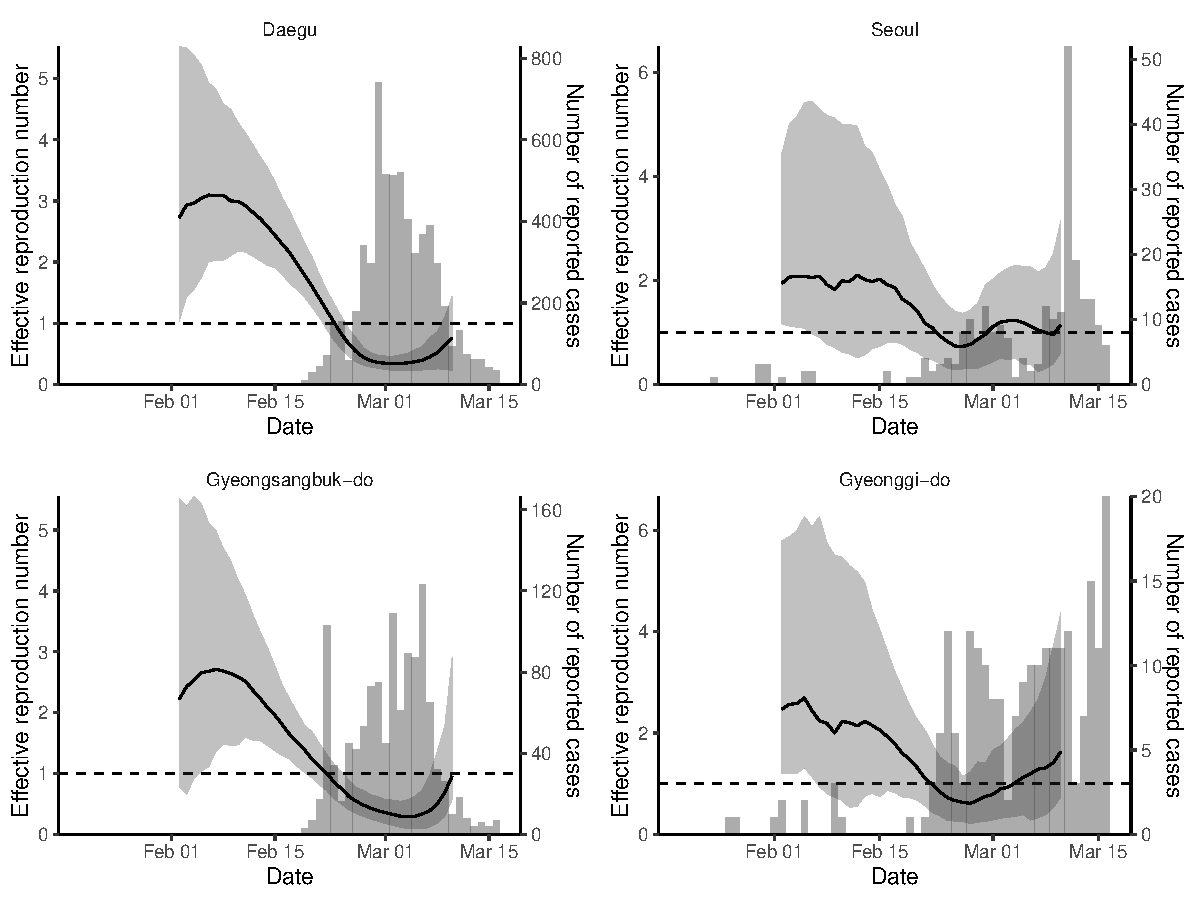
\includegraphics[width=\textwidth]{figure_R_t_all.pdf}
\caption{
\textbf{Comparison of effective reproduction number and the daily number of reported cases in Daegu, Seoul, Gyeongsangbuk-do, and Gyeonggi-do.}
}
\end{figure}

\pagebreak

\begin{figure}[!ht]
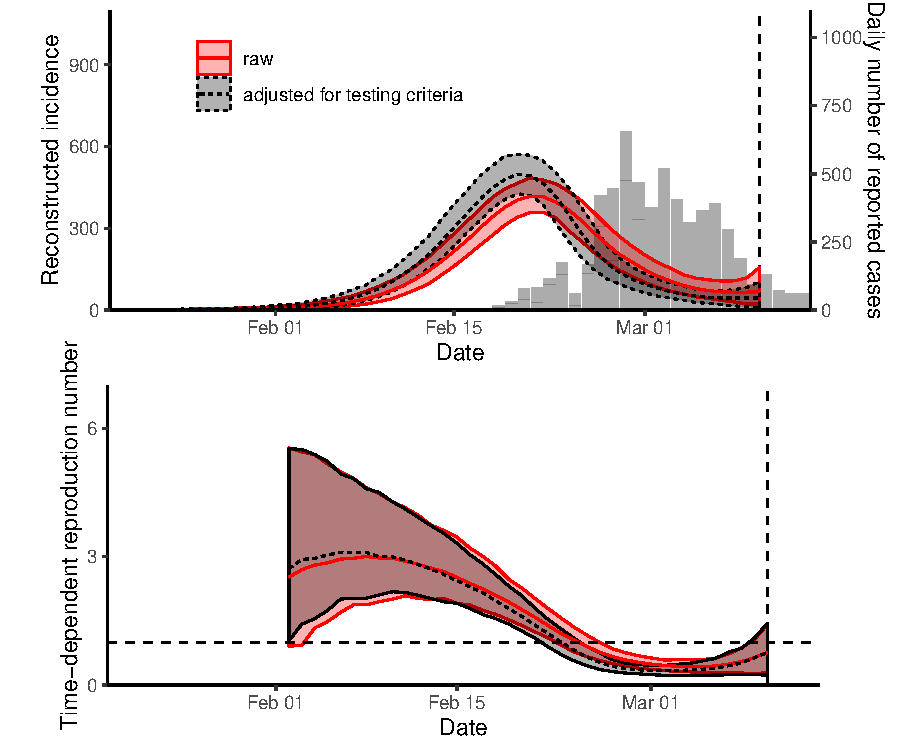
\includegraphics[width=\textwidth]{figure_R_t_daegu.pdf}
\caption{
\textbf{Sensitivity analysis of estimates of $\mathcal R_t$ in Daegu.}
}
\end{figure}

\pagebreak

\begin{figure}[!ht]
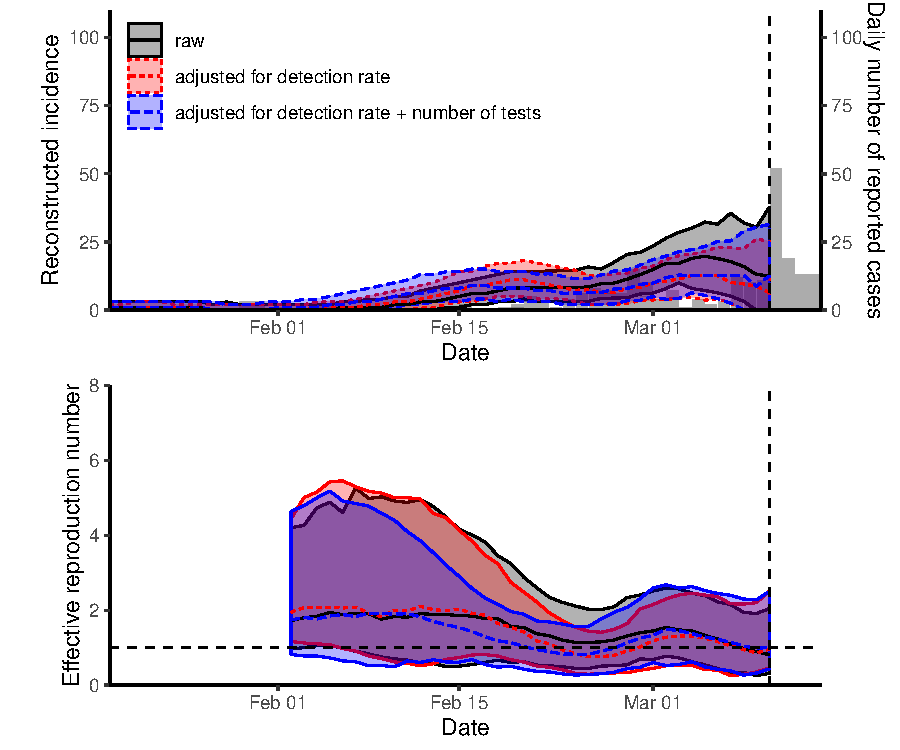
\includegraphics[width=\textwidth]{figure_R_t_seoul.pdf}
\caption{
\textbf{Sensitivity analysis of estimates of $\mathcal R_t$ in Seoul.}
}
\end{figure}

\pagebreak

\begin{figure}[!ht]
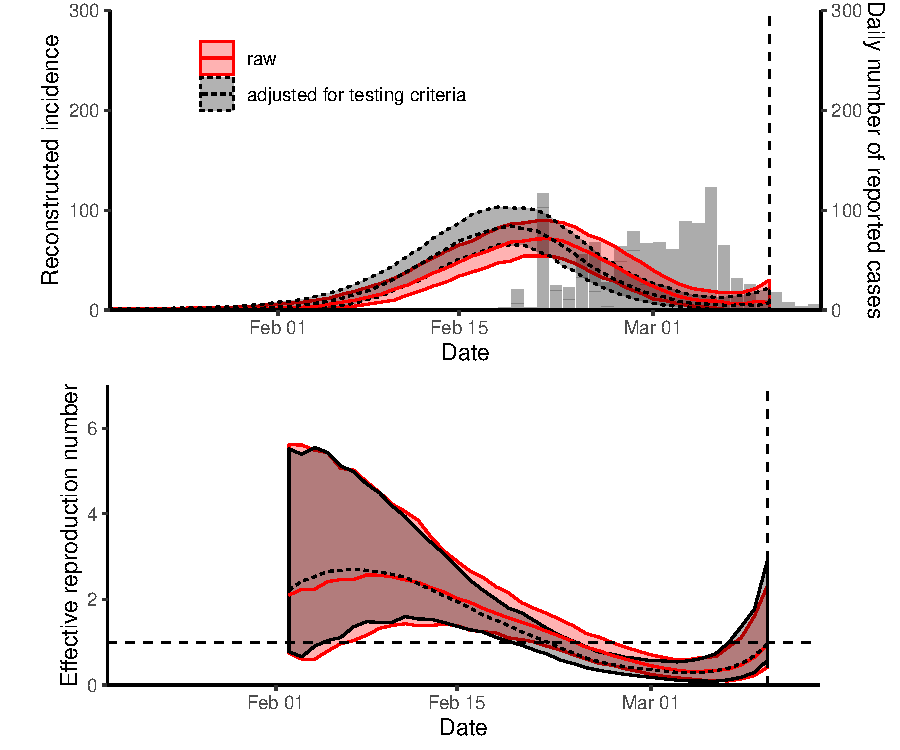
\includegraphics[width=\textwidth]{figure_R_t_gyeongbuk.pdf}
\caption{
\textbf{Sensitivity analysis of estimates of $\mathcal R_t$ in Gyeongsangbuk-do.}
}
\end{figure}

\pagebreak

\begin{figure}[!ht]
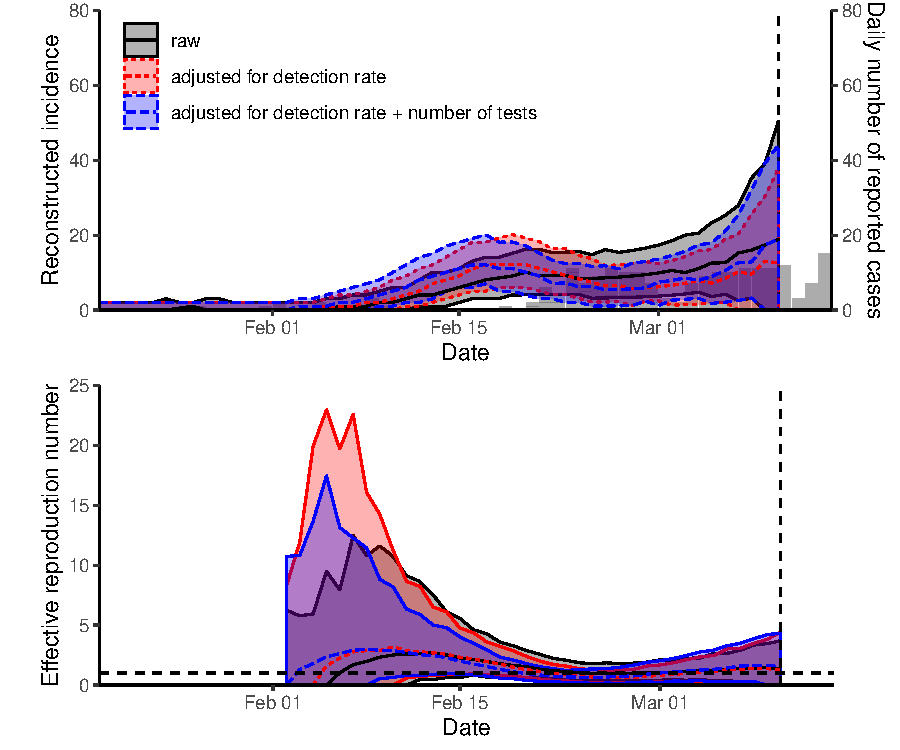
\includegraphics[width=\textwidth]{figure_R_t_gyeonggi.pdf}
\caption{
\textbf{Sensitivity analysis of estimates of $\mathcal R_t$ in Gyeonggi-do.}
}
\end{figure}

\pagebreak

\begin{figure}[!ht]
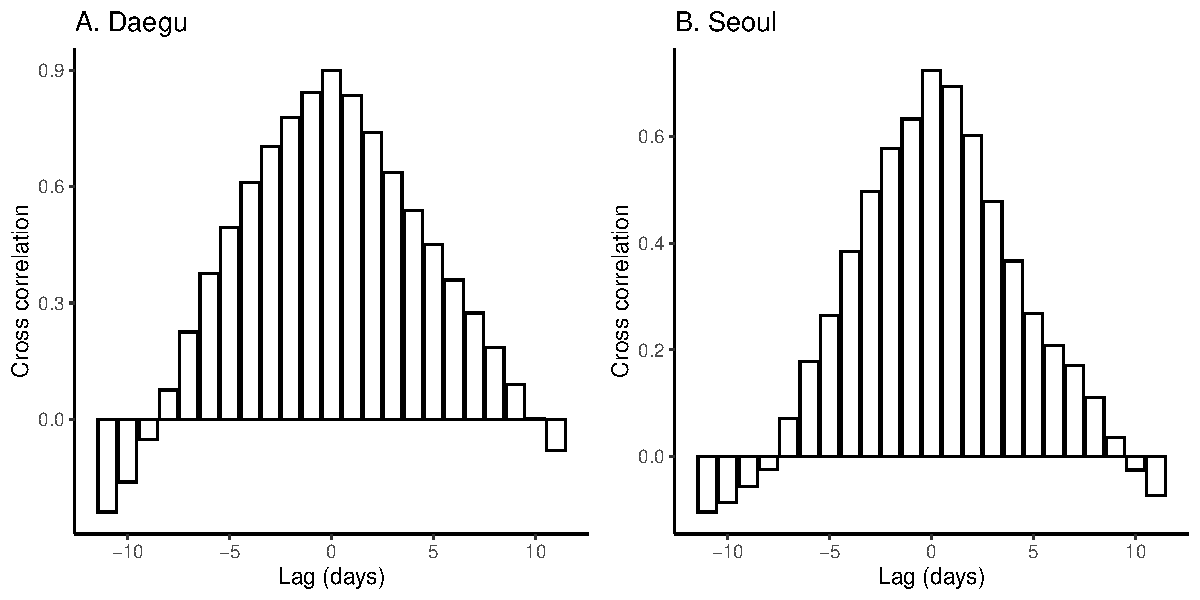
\includegraphics[width=\textwidth]{figure_cross.pdf}
\caption{
\textbf{Cross correlation between the normalized traffic volume and the median estimates of $\mathcal R_t$.}
}
\end{figure}

\end{document}
